\documentclass[border=6pt]{standalone}
\usepackage{tikz}
\usetikzlibrary{arrows.meta,calc,decorations.pathreplacing}
\begin{document}
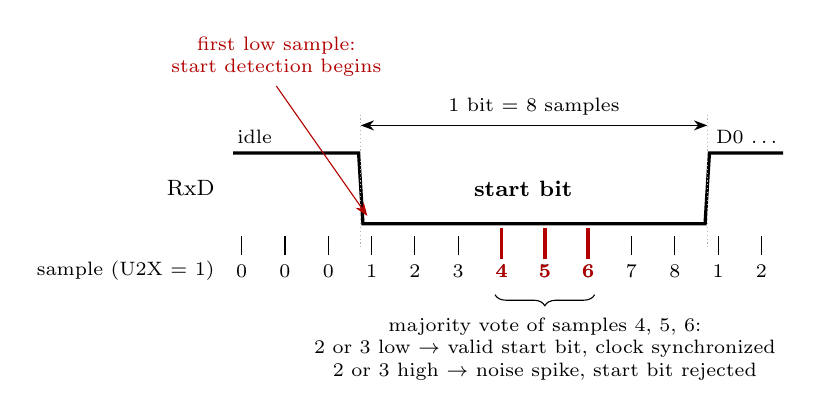
\begin{tikzpicture}[>=Stealth,font=\small,x=0.55cm,y=1cm]
% U2X = 1: 8 samples per bit; sample k of the start bit at x = k-1 (x = 0 is the first low sample)
\def\h{0.9}
\node[anchor=east,font=\footnotesize] at (-3.4,0.45) {RxD};
\draw[very thick] (-3.2,\h) -- (-0.3,\h) -- (-0.2,0) -- (7.7,0) -- (7.8,\h) -- (9.5,\h);
\node[font=\scriptsize,anchor=south] at (-2.7,\h) {idle};
\node[font=\footnotesize\bfseries] at (3.5,0.45) {start bit};
\node[font=\scriptsize,anchor=south] at (8.7,\h) {D0 \dots};
\draw[gray!60,densely dotted] (-0.25,-0.3) -- (-0.25,1.4);
\draw[gray!60,densely dotted] (7.75,-0.3) -- (7.75,1.4);
% samples
\foreach \x/\l in {-3/0,-2/0,-1/0} { \draw (\x,-0.4) -- (\x,-0.15); \node[font=\scriptsize,below] at (\x,-0.4) {\l}; }
\foreach \k in {1,...,8} {
  \pgfmathsetmacro{\x}{\k-1}
  \draw (\x,-0.4) -- (\x,-0.15);
  \node[font=\scriptsize,below] at (\x,-0.4) {\k};
}
\foreach \k in {4,5,6} {
  \draw[red!70!black,very thick] (\k-1,-0.45) -- (\k-1,-0.05);
  \node[font=\scriptsize\bfseries,red!70!black,below] at (\k-1,-0.4) {\k};
}
\foreach \x/\l in {8/1,9/2} { \draw (\x,-0.4) -- (\x,-0.15); \node[font=\scriptsize,below] at (\x,-0.4) {\l}; }
\node[anchor=east,font=\scriptsize] at (-3.4,-0.6) {sample (U2X = 1)};
\draw[decorate,decoration={brace,mirror,amplitude=4pt}] (2.85,-0.9) -- (5.15,-0.9) node[midway,below=5pt,font=\scriptsize,align=center]{majority vote of samples 4, 5, 6:\\2 or 3 low $\to$ valid start bit, clock synchronized\\2 or 3 high $\to$ noise spike, start bit rejected};
\draw[->,red!70!black] (-2.2,1.75) node[above,font=\scriptsize,align=center]{first low sample:\\start detection begins} -- (-0.1,0.1);
\draw[<->] (-0.25,1.25) -- (7.75,1.25);
\node[font=\scriptsize,anchor=south] at (3.75,1.25) {1 bit = 8 samples};
\end{tikzpicture}
\end{document}
